%--------------------------------  Preamble  -----------------------------------

\documentclass[UTF8]{article}

\usepackage[letterpaper, margin=1.1in]{geometry}
\usepackage{graphicx}               % to insert figures
\usepackage{xcolor}                 % colors for e-copies
\usepackage{subcaption}             % subfigures
\usepackage{placeins}               % Float barriers
\usepackage{hyperref}               % PDF hyperreferences
\usepackage{booktabs}
\usepackage{array}
\usepackage{caption}
\usepackage{rotating}

\newsavebox{\savefig}

\title{
  Outworlds Wastes\\
  ~\\
  \large BattleTech League Framework \\
  ~\\
  ~\\
  ~\\
  
\includegraphics[width=4in]{../img/Outworlds_Alliance.png}
}
\author{}
\date{}

% Optional PDF information
\ifpdf
\hypersetup{
  pdftitle={Outworlds Wastes},
  pdfauthor={Jeremy L Thompson}
}
\fi

%-------------------------------------------------------------------------------
%--------------------------------  Document  -----------------------------------
%-------------------------------------------------------------------------------

\begin{document}

\maketitle

\newpage

Outworlds Wastes is a casual BattleTech league framework with simplified logistics rules.
Players will take the role of commander of a mech force searching the Outworlds Wastes for lost technology and glory.
Completing objectives in scenarios will earn C-bills that commanders can use to upgrade their forces.
Different formats of scenario play are supported, to include Classic BattleTech, Alpha Strike, and BattleTech: Destiny.\\

\subsection*{Goals}

\begin{itemize}

\item Have lots of fun while fostering a friendly and welcoming environment.

\item Give players an opportunity to build personalized lore for their own mechwarrior forces.

\item Provide a lightweight framework for players to track the accomplishments of their forces.

\item Explore BattleTech lore and equipment.

\item Require minimal resources beyond \emph{BattleTech: Total Warfare} and the \emph{Master Unit List}.

\item Support players across a variety of experience levels.

\end{itemize}

\subsection*{Contents}

These rules cover four general areas: background information, player information, league organizer information, and reference material.\\

Background information on the Outworlds Wastes region and the overall design of the Outworlds Wastes league is in Chapter 1.
The new rules for players are in Chapter 2.
Force Construction rules, page 5, and Force Maintenance and Improvements rules, page 8, are the minimum rules needed to jump into Outworlds Wastes league play.
Rules for league organizers are found in Chapters 3 and 4.
Rules for scenario design and scoring are found in Chapter 3, and rules for league scoring are found in Chapter 4.
The remaining chapters contain supplemental reference material, to include a region map and sample tables for tracking a player's forces.\\

\newpage

\tableofcontents
\newpage

\section{Background}

The Outworlds Alliance was founded in 2413 and enjoyed prosperity throughout the Star League Era.
By the start of the Amaris Civil War in 2766, the Outworlds Alliance contained over 135 major systems across 7 administrative districts.
Unfortunately, the Outworlds Alliance suffered during the Succession Wars that followed the fall of the Star League in 2780, and they had to steadily abandon systems that they no longer had the resources to support.\\

Clan Snow Raven began exploring the Periphery for resources soon after the battle of Tukayyid ended Operation REVIVAL.
In 3064, Clan Snow Raven and the Outworlds Alliance began developing mutual respect and tentative alliance.
Following their abjuration from the Clan Homeworlds in 3075 as a result of the Wars of Reaving, Clan Snow Raven took refuge in the Outworlds Alliance.
In 3083, Clan Snow Raven and the Outworlds Alliance merged to form the Raven Alliance.
By the ilClan Trial in 3151, the Raven Alliance contained only 47 systems.\\

The exact number of systems varies from era to era, but approximately 88 systems that were part of the Outworlds Alliance during the Star League era have been lost.
These lost worlds form the Outworlds Wastes.
Many factions are eager to explore these lost worlds in the Outworlds Wastes in search of lost Star League technology or to take refuge from the complex political machinations of the Inner Sphere.\\

You will take the role of commander of a mech force exploring the Outworlds Wastes for your faction during the current league era.
Common factions for the region include

\begin{itemize}

\item Outworlds Alliance

\item Clan Snow Raven

\item Draconis Combine

\item Federated Suns

\item Mercenary groups

\item Pirate gangs

\item Clan Dark Caste

\end{itemize}

Commanders should pick the faction they are most interested in representing.
While the major factions are the most prevalent in the region, other factions may be found in the Outworlds Wastes.
For example, the Raven Alliance has relationships with nations on the far side of the Periphery, such as Magistracy of Canopus.\\

Commanders will compete with other factions in the Outworlds Wastes to grow their force and recover lost technology.
Scenarios are primarily designed for Classic BattleTech, but scenarios for Alpha Strike and BattleTech: Destiny is also supported.\\

League organizers pick the era for the current league; organizers can select any era after the fall of the Star League.
The era determines unit availability and the most common factions in the Outworlds Wastes.
Commanders should ask the league organizer which era is being used.\\

\newpage

\section{Force Management}

Unit commanders will start with Battle Value points (BV) budget they can use to purchase their initial units.
Participation in scenarios and accomplishing objectives will earn C-bills for commanders to spend on training their pilots, upgrading units, and acquiring new equipment.

\subsection{Force Construction}

Commanders start with 10,000 BV to acquire initial units for their force.
BV costs for all units are listed in the \href{http://www.masterunitlist.info}{Master Unit List}.
Force construction must follow these rules:\\

\begin{itemize}

\item Commanders have a modified Union class dropship with 16 configurable maintenance bays to hold their units.
Each bay can hold 1 mech, 2 combat vehicles, 5 protomechs, or 5 tons of infantry/battle armor.
Infantry/battle armor units can be split across multiple bays; for example, 4 bays can hold 20 tons, which is 5 squads of inner sphere standard battle armor.
The dropship can support a maximum of 12 mech bays, 5 combat vehicle, 2 protomech bays, and 5 infantry/battle armor bays.
You may leave bays unconfigured or change their configuration in the future.
Your entire force must fit onto your dropship.

\item Commanders should select units from their faction on the \href{http://www.masterunitlist.info/}{Master Unit List} for era chosen by league organizers.
Forces can include units with introductory, standard, and advanced technology but should not include experimental units.
For example, the Marauder MAD-3R, Marauder MAD-7R, and Marauder II MAD-6C are legal ilClan era mercenary units while the Marauder II MAD-6M is not.
Forces can include one unique unit of any technology level.

\item Each force can start with no more than 7,000 BV in mechs.
Commanders are encouraged to try to use the typical mech unit composition of their faction.
However, this can be difficult to accomplish for clan or ComStar forces, so this is not a requirement.

\item Each force can include any number of supporting units, such as combat vehicles, protomechs, battle armor, and infantry.
Some scenarios will require infantry or battle armor and combat vehicles with cargo capacity, so commanders should have at least one of each of these units in their force.

\item Forces cannot contain off-map battlefield support units, such as artillery or aerospace fighters.
However, forces can contain any on-map units.

\item The BV costs of a unit includes the skill levels.
Skill levels should generally be close to the average skill levels given on page 40 of \emph{BattleTech: Total Warfare}.
Initial skill levels for a unit may be no better than Gunnery 3/Piloting 4.

\item Any BV not spent during force creation is lost.

\end{itemize}

One of the goals of the Outworlds Wastes framework is to explore different equipment.
Commanders are encouraged to know where in the rule books other commanders can read about the rules pertaining to any special equipment for units in their force.
Unit record sheets for these units can be generated found using \href{https://megamek.org}{MegaMekLab} or similar tools.\\

Learning new types of units can be intimidating, especially in Classic BattleTech.
Commanders are welcome to limit the number of types of units in their 3,000 BV non-mech forces.
For example, a force could include only troop transports and battle armor so the commander can meet any objective while keeping new rules to a minimum.\\

Two sample initial forces are provided; the first force is a Civil War era mercenary company and the second force is an ilClan era Raven Alliance nova.
Mech pilot names are encouraged, as one of the goals is to develop the personalized lore for your force.\\

\newpage

\begin{table}[h!]
\centering
\newcolumntype{R}[1]{>{\raggedleft\let\newline\\\arraybackslash\hspace{0pt}}m{#1}}
\begin{tabular}{| m{1.25em} m{11em} m{8em} R{3.85em} R{3.85em} R{3.5em} R{3.5em} |}
\hline
Bay & Unit                  & Pilot            & Gunnery & Piloting & BV    & Adj BV \\
\hline
\multicolumn{7}{|c|}{Mechs} \\
\hline
1   & Atlas II AS7-D        & 'Meg' Courant    & 3       & 4         & 1,897 & 2,504 \\
2   & Phoenix Hawk PXH-2K   & 'Bison' Helge    & 4       & 5         & 1,271 & 1,271 \\
3   & Blackjack BJ-2        & 'Lizard' Baker   & 4       & 5         & 1,148 & 1,148 \\
4   & Locust IIC            & 'Casper' Poole   & 4       & 5         & 1,100 & 1,100 \\
\hline
\multicolumn{7}{|c|}{Combat Vehicles} \\
\hline
1  & Maxim Hover Transport &                   & 4       & 5         &   764 &   764 \\
1  & Maxim Hover Transport &                   & 4       & 5         &   764 &   764 \\
2  & Galleon GAL-102       &                   & 4       & 5         &   651 &   651 \\
2  & Galleon GAL-102       &                   & 4       & 5         &   651 &   651 \\
3  & Warrior H-7           &                   & 4       & 5         &   295 &   295 \\
3  & Warrior H-7           &                   & 4       & 5         &   295 &   295 \\
\hline
\multicolumn{7}{|c|}{Infantry/Battle Armor} \\
\hline
1  & IS Std BA, LRR        &                   & 4       & 5         &   255 &   255 \\
2  & IS Std BA, Laser      &                   & 4       & 5         &   231 &   231 \\
\hline
9  & Total Bays            &                   &         &           &       &       \\
   & Total BV              &                   &         &           &       & 9,929 \\
\bottomrule
\end{tabular}
\caption{Civil War Era Mercenary Force - Meg's Magpies}
\end{table}

\begin{table}[h!]
\centering
\newcolumntype{R}[1]{>{\raggedleft\let\newline\\\arraybackslash\hspace{0pt}}m{#1}}
\begin{tabular}{| m{1.25em} m{11em} m{8em} R{3.85em} R{3.85em} R{3.5em} R{3.5em} |}
\hline
Bay & Unit                  & Pilot           & Gunnery & Piloting  & BV    & Adj BV \\
\hline
\multicolumn{7}{|c|}{Mechs} \\
\hline
1   & Carrion Crow A        & Sarah Magnus    & 3       & 4         & 1,622 & 2,141 \\
2   & Nova U                &       Bryn      & 4       & 5         & 1,413 & 1,413 \\
3   & Adder J               &       Ada       & 4       & 5         & 1,222 & 1,222 \\
4   & Kit Fox V             &       Soton     & 3       & 4         &   974 & 1,286 \\
5   & Fire Moth A           &       Tina      & 3       & 4         &   639 &   843 \\
\hline
\multicolumn{7}{|c|}{Combat Vehicles} \\
\hline
1   & Karnov UR Transport   &                 & 4       & 5          &   125 &   125 \\
\hline
\multicolumn{7}{|c|}{Infantry/Battle Armor} \\
\hline
1   & Gnome BA              &                 & 3       & 4         &   580 &   766 \\
2   & Elemental BA, Laser   &                 & 3       & 4         &   447 &   590 \\
3   & Elemental BA, HMG     &                 & 3       & 4         &   415 &   548 \\
4   & Elemental BA, Flamer  &                 & 3       & 4         &   404 &   533 \\
5   & Elemental BA, Flamer  &                 & 3       & 4         &   404 &   533 \\
\hline
11  & Total Bays            &                 &         &           &       &       \\
    & Total BV              &                 &         &           &       & 10,000 \\
\hline
\end{tabular}
\caption{ilClan Era Raven Alliance Force - Raven Expeditionary Cluster, Alpha Nova}
\end{table}

Both forces can support additional units on their dropships.
However, the Raven Expeditionary Cluster, Alpha Nova force cannot support any additional infantry/battle armor maintenance bays because their dropship is using the maximum of 5 bays.\\

\newpage

\subsection{Advanced Force Construction Rules}

The \href{http://www.masterunitlist.info/}{Master Unit List} provides all factions from official BattleTech lore.
A commander can create a modified faction list representing their custom faction.\\

To create a custom faction list, go to the \href{http://www.masterunitlist.info/Unit/Filter}{Units Tab on Master Unit List}.
Filter the units to include one faction list and one general list.
For example, the Pirates faction by default typically includes the Periphery General list.
A Dark Caste custom faction might include the Pirates faction list with the Inner Sphere Clan General list.\\

Be sure to also filter by the appropriate Availability Era.
All other restrictions from the basic Force Construction rules, such as era and technology level, still apply.\\

Any faction that has a general list can be modified with these rules.
If the faction does not have a general list, then it cannot be customized in this way.
Factions without a general list include Mercenary, Kell Hounds, Wolf's Dragoons, and Society.
These factions have the phrase "including Blank General List" on their faction and era specific page.
Adding a general list to these factions would give the commander a disproportionately large number of units to choose from.\\

Commanders can create a custom mercenary faction with these Advanced Force Construction Rules.
First select a faction list for the region in which the force was founded or primarily operates and then pick an appropriate general list.
For example, a mercenary force that was founded in the Draconis Combine but moved to the Periphery after Coordinator Takashi Kurita's \emph{Death to Mercenaries} edict could use Draconis Combine faction list with the Periphery General list.\\

\begin{figure}[h!]
  \centering
  \begin{subfigure}{0.4\textwidth}
    \centering
    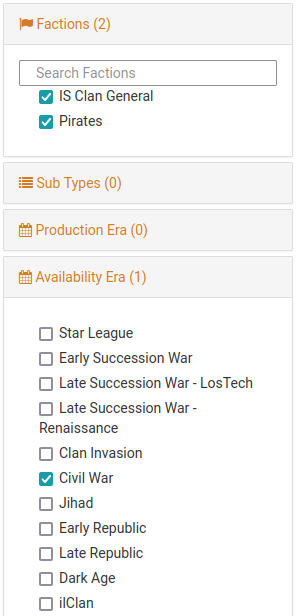
\includegraphics[height=3.8in]{../img/Dark_Caste_List.png}
    \caption{Dark Caste Faction}
  \end{subfigure}
  \hspace{1in}
  \begin{subfigure}{0.4\textwidth}
    \centering
    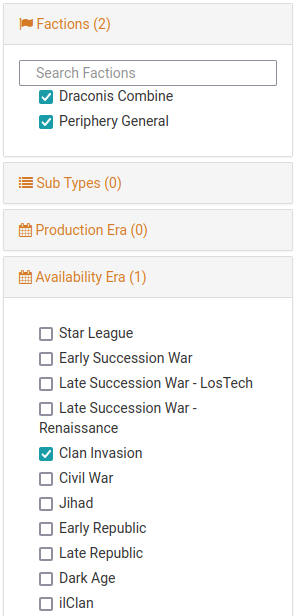
\includegraphics[height=3.8in]{../img/Combine_Mercenary_List.png}
    \caption{Combine Mercenary Faction}
  \end{subfigure}
  \caption{Custom Faction Lists}
\end{figure}

\newpage

\subsection{Force Maintenance and Improvements}

After earning C-bills from scenarios, commanders can spend C-bills to improve their force.
Possible improvements are listed below.
C-bill costs for all units are listed in the \href{http://www.masterunitlist.info}{Master Unit List}.\\

\begin{itemize}

\item {\bf Train}: Pay 500,000 C-bills multiplied by the difference in BV skill multiplier to improve a unit's skill levels.
For example, a Gunnery 4/Piloting 5 pilot has a BV skill multiplier of 1.0 and a 3/4 pilot has a BV skill multiplier of 1.32.
Therefore, it costs 160,000 C-bills to train a 4/5 pilot to be a 3/4 pilot.
Any unit cannot be upgraded past 1/2.
New or replaced units cannot be upgraded past 3/4.
Existing units that did not participate in the most recent scenario cannot be upgraded past 4/5.
See \emph{BattleTech: Techmanual}, page 315, for the BV skill multiplier table.
A unit's skill levels can be degraded at no C-bill cost, but future improvements will still cost C-bills.

\item {\bf Replace}: Pay 50\% of the C-bill cost, rounded up, to replace a \emph{destroyed} unit.
If the mech pilot or vehicle crew was killed, the replacement cost includes a 5/6 pilot or crew.
If an entire infantry or battle armor unit was destroyed, the replacement cost includes 5/6 troops.
The protomech replacement cost includes a 5/6 pilot.
The new unit can be trained as above.
See \emph{BattleTech: Total Warfare} for the definition of \emph{destroyed} for different types of units.

\item {\bf Repair}: Pay 25\% of the C-bill cost, rounded up, to repair all internal damage and critical components for a mech, protomech, or combat vehicle that has not been \emph{destroyed}.
If the pilot or crew was killed, the repair cost includes a 5/6 pilot or crew.
Armor repairs have no C-bill cost.

\item {\bf Recruit}: Pay 50\% of the C-bill cost, rounded up, recruit new troops to replace troops in an infantry or battle armor unit that has not been \emph{destroyed}.
For example, if 1 out of 4 troops was killed in a battle armor squad, pay 50\% of the C-bill cost for 1 suit.
To replace 1 troop in a squad of 4 IS Standard Battle Armor with Lasers, pay 293,125 C-bills.
Damage to battle armor troops that survive a scenario is repaired for free.

\item {\bf Refit}: Pay the difference in C-bill cost to refit a unit to a different variant.
A Phoenix Hawk PXH-2 costs 4,348,840 C-bills and a Phoenix Hawk PXH-1K costs 3,628,553.
A commander may pay 720,287 C-bills to convert a PHX-2 into a PHX-1K or to convert a PHX-1K into a PHX-2.
Note that it still costs C-bills to refit when the new variant is cheaper.

\item {\bf Omni Refit}: Omnimechs can be temporarily converted to a cheaper variant for a scenario for free, but refitting is required to use more expensive variants.
For example, the Carrion Crow C is worth 10,336,492 C-bills.
The Carrion Crow A only costs 9,704,829 C-bills, so a Carrion Crow C can be temporarily configured as a Carrion Crow A for a scenario.
However, a Carrion Crow B costs 15,617,992 C-bills, so a Carrion Crow C would need a 5,281,500 C-bill refit to be converted to the Carrion Crow B variant.
Once the Carrion Crow C is refitted to a Carrion Crow B, the omnimech can be configured as a Carrion Crow A, B, or C for any scenario.

\item {\bf Purchase}: Pay the C-bill cost to get a new unit.
Commanders should purchase units from their \href{http://www.masterunitlist.info}{Master Unit List} faction and era list.
The new unit starts at skill 4/5 and can be trained.

\item {\bf Salvage}: Pay 50\% the C-bill cost, rounded up, to salvage units that you destroyed in a scenario.
A War Crow Prime costs 22,057,358 C-bills, and a salvaged War Crow Prime costs 11,028,679 C-bills.
Salvage is the primary way for commanders to get units that are not on their \href{http://www.masterunitlist.info}{Master Unit List} faction and era list.
The new unit starts at skill 4/5 and can be trained.

\item {\bf Sell}: Commanders can sell units for 50\% of the C-bill cost or destroyed units for 25\% of the C-bill cost, rounded up.
A Locust LCT-1E costs 1,574,200 C-bills and can be sold for 787,100 C-bills.
If the Locust LCT-1E was destroyed, then selling it would only yield 393,550 C-bills.
Commanders can earn 25\% of the C-bill cost for selling a salvaged unit instead of paying 50\% of the C-bill cost to repair the unit.
A salvaged War Crow Prime could be sold to earn 5,514,340 C-bills instead of paying 11,028,679 C-bills to repair it.

\end{itemize}

\newpage

\subsection{Advanced Force Maintenance and Improvements}

Commanders may use these advanced rules to further improve their force.

\begin{itemize}

\item {\bf Retrain}: When selling a unit and immediately purchasing a replacement unit of the same type, commanders may retrain the old pilot/crew for the new unit.
Pay 250,000 C-bills multiplied by the difference in BV skill multiplier between their current skill level and 4/5 to retrain the crew/pilot.
For example, a 3/3 pilot has a BV skill multiplier of 1.44.
Therefore, it costs 110,000 C-bills to retrain a 3/4 pilot for a new unit.
See \emph{BattleTech: Techmanual}, page 315, for the BV skill multiplier table.
The old and new unit must be the same type.
For example, a mech pilot can only be retrained into another mech unit.
A combat vehicle crew can only retrain to the same type of combat vehicle: ground, VTOL, WiGE, or naval.
See \emph{BattleTech: Total Warfare}, page 192, for discussion of the combat vehicle types.

\item {\bf Quirks}: Commanders may customize their units with quirks.
Pay 10\% of the unit's cost in C-bills per positive quirk point to add a positive quirk.
For each positive quirk, commanders must select a negative quirk of equal or higher point value.
These quirks should generally match the lore and common quirks for the unit.
See \emph{BattleTech: Battlemech Manual}, page 82, or \emph{BattleTech: Campaign Operations}, page 225, for a list of all quirks.
See \emph{BattleTech: Battlemech Manual}, page 90, for a table of typical quirks for each mech and see \emph{BattleTech: Campaign Operations}, page 255, for table summarizing which quirks may be applied to which unit types.
Some quirks require modifications to fit in the Outworlds Wastes rules.

\begin{itemize}

\item Two mechs with the \emph{Compact 'Mech} quirk may share a dropship bay.

\item Quirks that modify maintenance rolls, such as \emph{Easy to Maintain} and \emph{Difficult to Maintain} instead reduce or increase the base cost for calculating repair and replacement costs by 10\%.

\item \emph{Good Reputation} costs 1 point.

\item The \emph{Modular Weapons} quirk reduces the Refit cost by 50\%.

\end{itemize}

\end{itemize}

\newpage

\section{Scenarios}

Commanders earn C-bills to spend on their forces through participation in scenarios and accomplishing objectives.
Scenarios will often be built to represent lore and objectives relevant to specific worlds in the Outworlds Wastes.
Scenarios may include special bonuses, such as recovering equipment from the 61st Royal Jump Infantry Division so a commander can add advanced jump infantry to their force.

\subsection{Scenario Formats}

Outworlds Wastes forces are created and tracked using Classic BattleTech BV values, but scenarios can be played in many formats.
Common formats for the scenarios include

\begin{itemize}

\item {\bf Classic BattleTech}: Scenarios for this format will primarily focus on medium scale combat, with each side controlling approximately one lance with supporting assets.

\item {\bf Alpha Strike}: Scenarios for this format will primarily focus on large scale combat, with each side controlling approximately one company with supporting assets.

\item {\bf BattleTech: Destiny}: Scenarios for this format will focus on small scale combat, with each side controlling approximately one or two mechs.

\end{itemize}

Regardless of the scenario format, force maintenance and improvement costs are always calculated per Section 3.3 above.
Use the rules for the scenario format to define terms such as \emph{destroyed}, \emph{internal damage}, and \emph{critical damage}.\\

Unit Alpha Strike cards are available on the \href{http://www.masterunitlist.info}{Master Unit List}.
To convert a unit skill levels from Classic BattleTech to Alpha Strike, take the average of the piloting and gunnery skills, rounded down.
See \emph{Alpha Strike: Commander's Edition}, page 29.\\

BattleTech: Destiny is a rule system that combines MechWarrior Destiny RPG and Alpha Strike combat rules while drawing some inspiration from Classic BattleTech.
BattleTech: Destiny rules and record sheets can be created on the \href{https://dfawargaming.com}{Death From Above Wargaming} website.

\subsection{Scenario Forces}

Both sides should agree upon a BV (or Point Value, PV) and unit count limit before starting the scenario.
A typical BV limit would be 6,000 BV per side for 1v1 or 10,000 BV per side for 2v2.
A typical PV limit would be 150 PV per side for 1v1 or 250 PV per side for 2v2.
A typical unit limit depends upon the format but would be approximately 7 units per side for 1v1 or 10 units per side for 2v2.
Additional limits on specific unit types, such as 2 infantry/battle armor units per side, can be imposed as well.\\

Scenarios can be played with higher BV or PV limits, but C-bills awarded should be adjusted if the limits are significantly higher.
For example, an Alpha Strike 300 PV per side 1v1 scenario could have its C-bills awarded doubled compared to a Classic BattleTech 6,000 BV per side 1v1 scenario.\\

To simplify scoring, Alpha Strike scenarios may be played with BV limits instead of PV limits.
Commanders would select units to meet the BV limit and use the Alpha Strike cards and rules for the scenario.

\subsection{Scenario Balancing}

One of the goals for the Outworlds Wastes league framework is to foster a friendly and welcoming environment.
A mix of experience levels between commanders is expected.
We propose some options to help balance scenarios so game play is welcoming while also staying fresh and challenging.\\

\begin{itemize}

\item {\bf Setup}: When setting up a scenario, slight preference should generally be given to the commander whose force has the lower total BV, including all units and pilots.
For example, the commander with the lowest total BV could be offered the choice between attacking and defending for the casual scenarios given below.
For a scenario with a terrain setup phase, the commander with the lowest total BV could be offered the first placement of terrain piece.

\item {\bf 2v2}: Many scenarios are described as 1v1; however these scenarios can often support 2v2 or similar play.
When playing on teams, experience should be divided roughly equally between the two teams.
Teammates are encouraged to collaborate on strategy for the scenario.

\end{itemize}

\subsection{Scenario Scoring}

Scenarios award C-bills in two ways, through participation and completing objectives.
The C-bills awarded in a scenario will tend to follow these guidelines

\begin{itemize}

\item {\bf Objectives}: Forces earn 7,000,000 C-bills for completing primary objectives and 3,000,000 C-bills for completing secondary objectives.
This C-bill payment represents bonus pay in a mercenary contract and the value of resources or technology acquired by completing mission objectives.

\item {\bf Base Pay}: If the force did not complete any objectives, then the force earns 2,000 C-bills for every 10 BV for the scenario, with a minimum of 1,000,000 C-bills.
For example, a 6,000 BV vs 6,000 BV scenario will have a base payout of 1,200,000 C-bills.
This C-bill payment represents the baseline cost of a mercenary contract or supplies sent by a faction.

\end{itemize}

\subsection{Casual Scenarios}

While there are scenarios provided by the league organizers, the Outworlds Wastes framework also supports scoring casual games between commanders to give their forces more chances to earn C-bills and glory.
Some primary and secondary objectives are included here as examples.\\

\subsubsection{Primary Objectives}

\begin{enumerate}

\item Extraction: The attackers select a hex within 5 rows of the defenders home edge.
This hex contains a target to extract.
A unit with cargo capacity can pick up the target by being in the same hex at the end of the turn.
The target is not destroyed if the carrying unit is destroyed.
A unit completes the objective by exiting their home edge while carrying the target.

\item King of the Hill: A hex in the center of the map contains a building with valuable files.
The building is medium with a construction factor of 60, unless the players agree upon a different configuration.
The force earns 1,000,000 C-bills for every turn that they have an infantry/battle armor unit inside of the building at the end of the turn.

\item Supply Raid: 3-7 supply depots are on the map, near the center.
Any unit with hands or cargo capacity can load supplies from the depot if they end their turn in the same hex.
A unit carrying supplies in their hands cannot fire any arm mounted weapons.
A unit carrying supplies earns a portion of 7,000,000 C-bills for bringing the supplies to their home edge.
Each side cannot score from the same supply depot twice until they score from every other supply depot.

\item Recovery: 4-6 disabled mechs are equally spaced along the map diagonal.
A mech of equal or higher weight class can drag a disabled mech.
To start dragging a disabled mech, a friendly mech must end the turn in the same hex as the disabled mech.
The dragging mech has a one half reduction in their walking MP, cannot jump, and cannot fire any weapons on its arm used for dragging.
A unit earns a portion of 7,000,000 C-bills for dragging a disabled mech to its home map edge.

\item Reconnaissance: The map contains 15 buildings that are at least hex large, 7 of which contain hidden objectives.
The attacker earns 1,000,000 C-bills for each hidden objective they find.
The defender earns 1,000,000 C-bills for each hidden objective the attacker does not find.

\item Assassination: A local militia commander needs to be escorted across the battlefield.
The defender selects a medium or heavy mech from the Periphery General or Pirates list.
The militia commander pilots this mech and must transit the map from the defender's home edge to the attacker's home edge.
The attacker earns 7,000,000 C-bills if the commander's mech is destroyed or 3,500,000 C-bills if the commander's mech receives crippling damage.
The defender 7,000,000 C-bills if the commander's mech does not receive crippling damage or if the commander's mech is crippled but not destroyed.

\end{enumerate}

\subsubsection{Secondary Objectives}

\begin{enumerate}

\item Cripple or destroy a mech.

\item Cripple or destroy a combat vehicle.

\item Destroy an internal section of an opponent's highest BV unit.

\end{enumerate}

\newpage

\section{League Play}

League play consists of two phases, Casual Play and Scoring.

\subsection{Casual Play Phase}

The Casual Play Phase gives commanders the opportunity to play casual scenarios and earn C-bills to upgrade their forces.
In this phase, scenarios may be 1v1 or 2v2.
After each casual scenario, the players can repair and update their forces per the Force Maintenance and Improvements rules.
At any point during this phase, a new commander can join the league or a current commander replace their force with a new one.
Any new force must follow the Force Construction rules.\\

This phase can last several months, and it can run concurrently with other events or leagues.
Commanders should keep track of the outcomes of all scenarios and all changes to their force, such as with the sample record sheets at the end of this packet.
Some additional restrictions may be enforced by league organizers, such as league play only occurring at a specific location.

\subsection{Scoring Phase}

During this phase, commanders play a series of narrative focused scenarios in a Swiss-system tournament.
The last scenario should be a large scale event that requires a significant portion of each commander's forces.
In this phase, scenarios may only be 1v1.
Each commander should play a different opponent during each scenario, if possible.
For each 1,000,000 earned during a scenario, the commander earns 1 point for scoring.
The players rankings are updated after each scenario.
Ties are broken by the the lowest total BV lost across all scenarios thus far, which \emph{destroyed} units counting as their full BV and units in \emph{forced withdrawal} counting as half their full BV.\\

At the end of these scenarios, winners are determined by their ranking.
Additional winners may be determined for specific categories, such as Best Painted Force or Best Force Lore.

\newpage

\section{Outworlds Wastes Map - ilClan Era}

\begin{figure}[h!]
  \centering
  \savebox{\savefig}{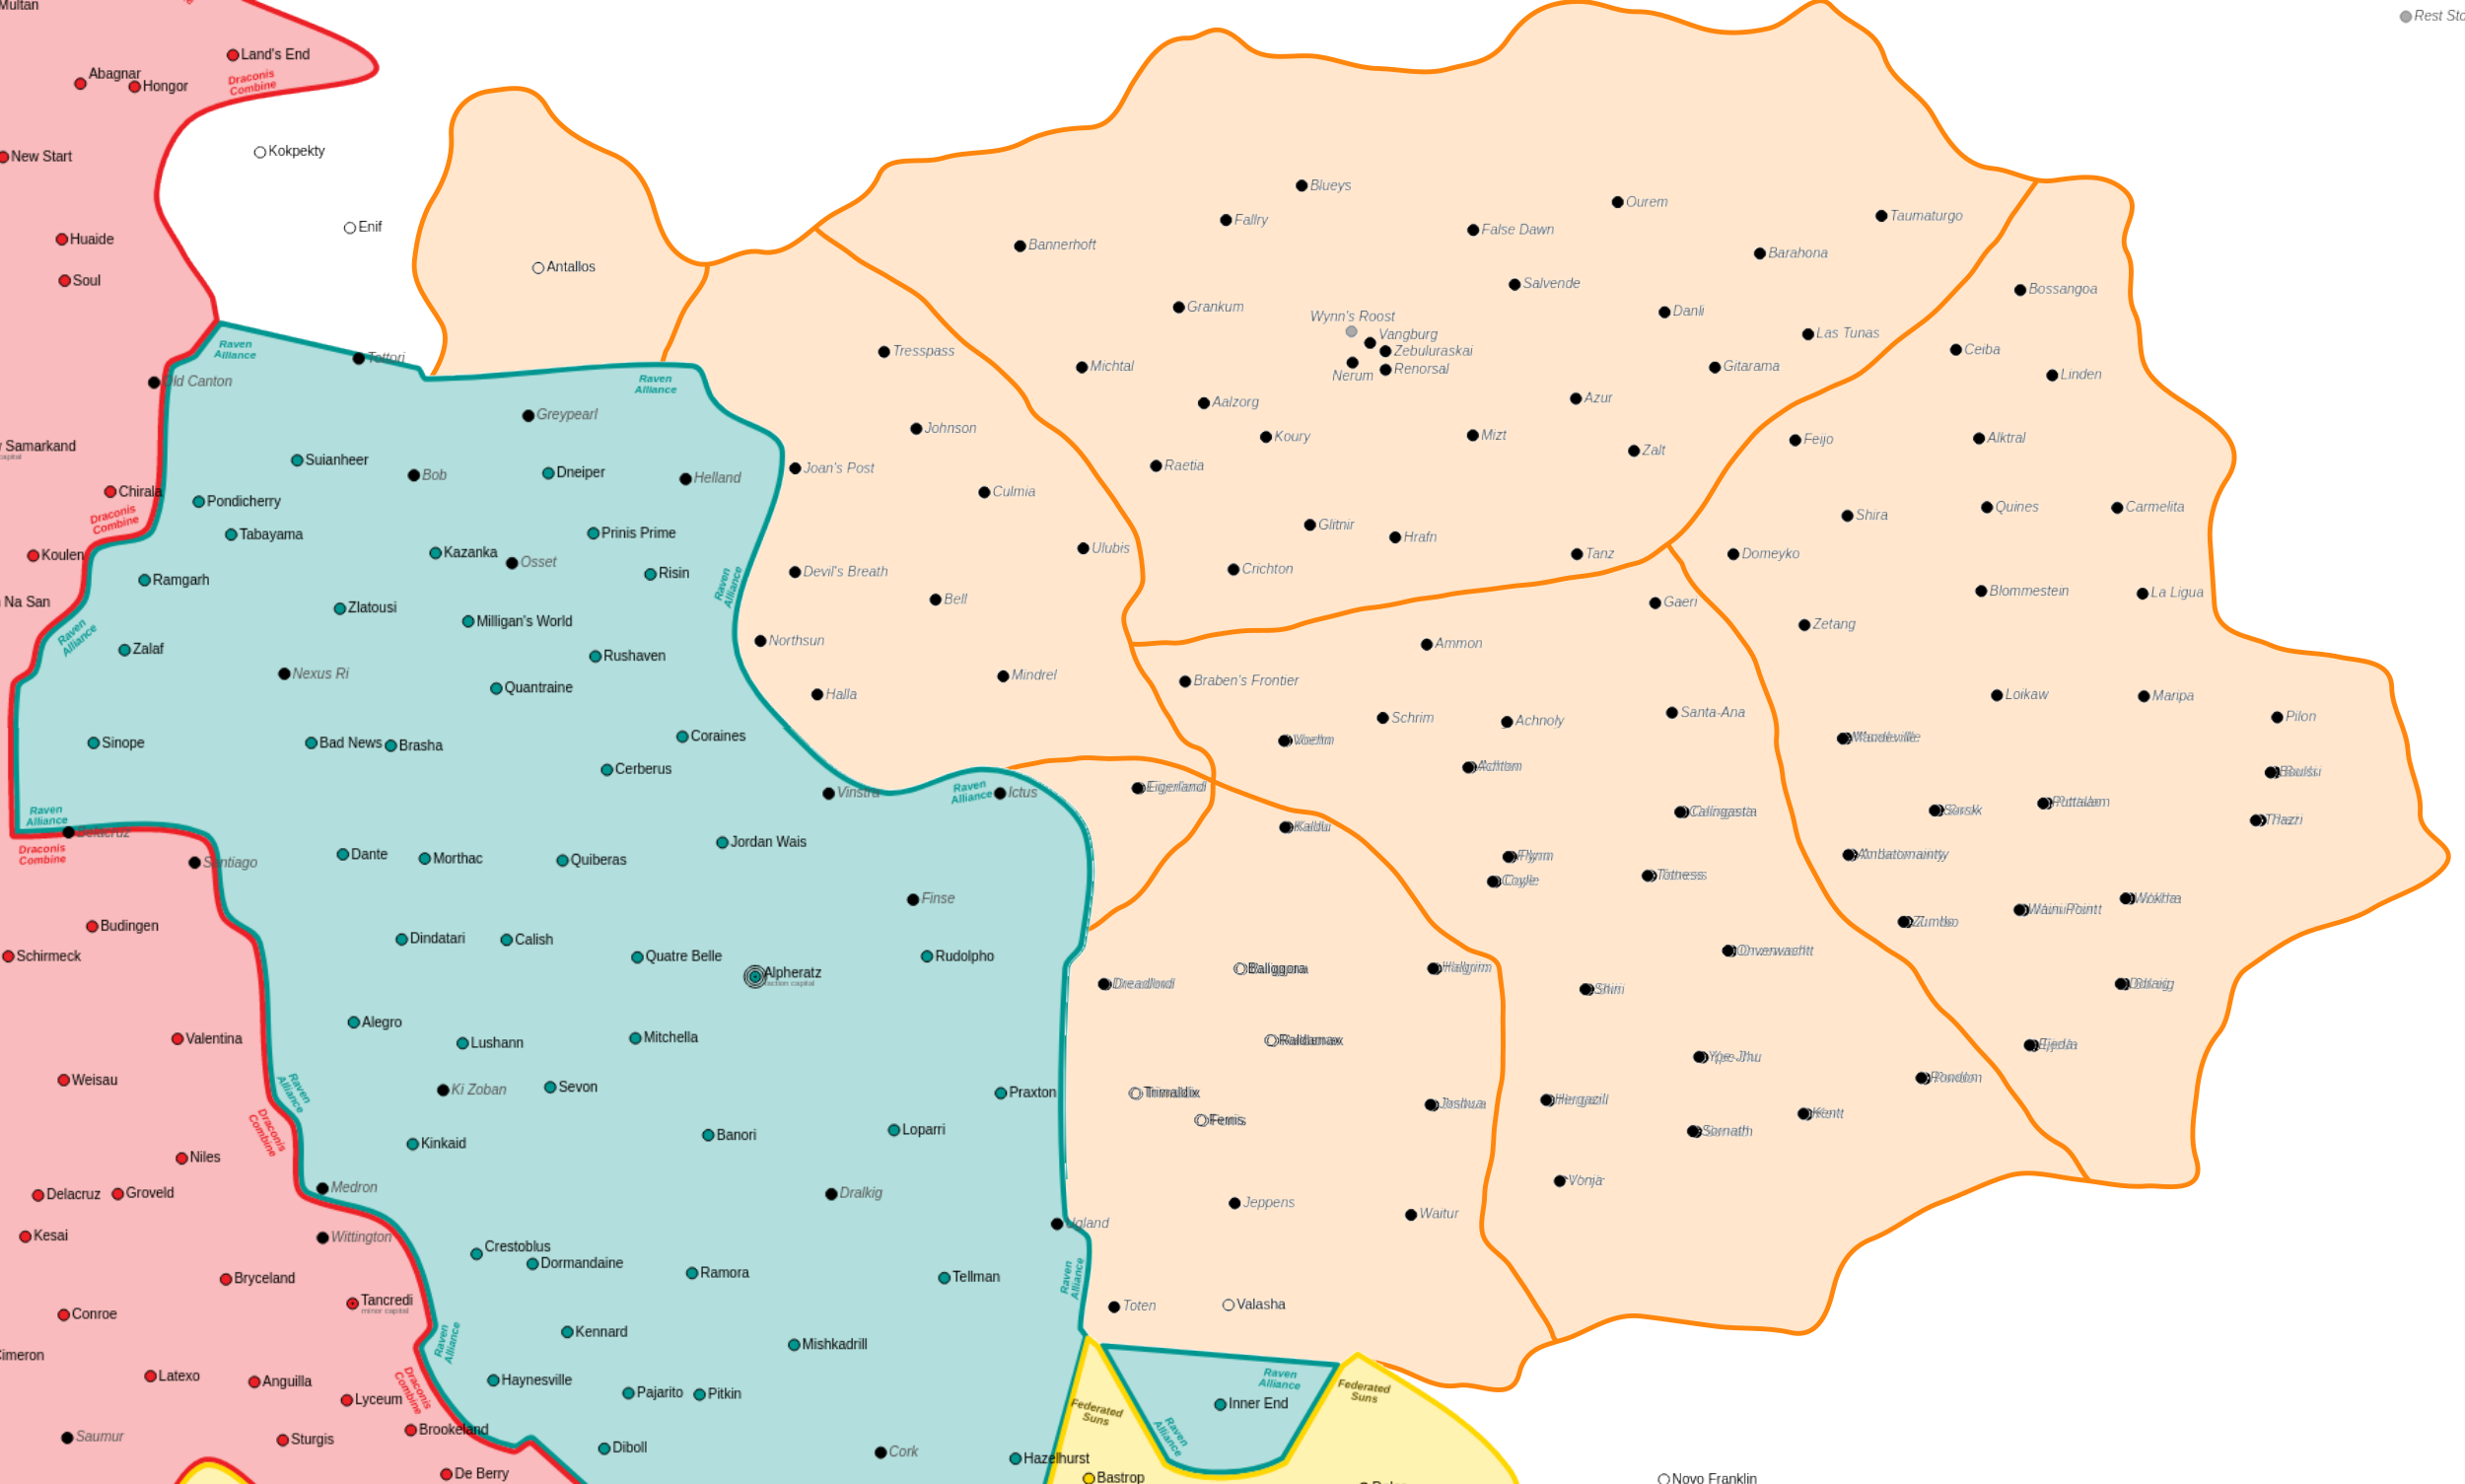
\includegraphics[width=8.1in]{../img/Outworlds_Wastes_ilClan_Map.png}}
  \rotatebox{90}{%
    \begin{minipage}{\wd\savefig}
      \usebox{\savefig}
      \caption{Outworlds Wastes - 3151}
    \end{minipage}}
\end{figure}

\newpage

\section{Sample Force Roster}

\begin{table}[h!]
\centering
\newcolumntype{R}[1]{>{\raggedleft\let\newline\\\arraybackslash\hspace{0pt}}m{#1}}
\begin{tabular}{| m{1.25em} m{11em} m{8em} R{3.85em} R{3.85em} R{3.5em} R{3.5em} |}
\hline
Bay & Unit & Pilot & Gunnery & Piloting & C-bills & BV \\
\hline
\multicolumn{7}{|c|}{Mechs (1 per bay)} \\
\hline
1  & & & & & & \\
2  & & & & & & \\
3  & & & & & & \\
4  & & & & & & \\
5  & & & & & & \\
6  & & & & & & \\
7  & & & & & & \\
8  & & & & & & \\
9  & & & & & & \\
10 & & & & & & \\
11 & & & & & & \\
12 & & & & & & \\
\hline
\multicolumn{7}{|c|}{Combat Vehicles (2 per bay)} \\
\hline
1 & & & & & & \\
1 & & & & & & \\
2 & & & & & & \\
2 & & & & & & \\
3 & & & & & & \\
3 & & & & & & \\
4 & & & & & & \\
4 & & & & & & \\
5 & & & & & & \\
5 & & & & & & \\
\hline
\multicolumn{7}{|c|}{Protomechs (5 per bay)} \\
\hline
1 & & & & & & \\
1 & & & & & & \\
1 & & & & & & \\
1 & & & & & & \\
1 & & & & & & \\
2 & & & & & & \\
2 & & & & & & \\
2 & & & & & & \\
2 & & & & & & \\
2 & & & & & & \\
\hline
\multicolumn{7}{|c|}{Infantry/Battle Armor (5 tons per bay)} \\
\hline
1  & & & & & & \\
2  & & & & & & \\
3  & & & & & & \\
4  & & & & & & \\
5  & & & & & & \\
...   & & & & & & \\
\hline
  & Total Bays (16 max) & & & & & \\
  & Total BV   & & & & & \\
\hline
\end{tabular}
\caption{Sample Force Roster}
\end{table}

\newpage

\section{Sample Scenario Logistics Tracking}

\begin{table}[h!]
\centering
\newcolumntype{R}[1]{>{\raggedleft\let\newline\\\arraybackslash\hspace{0pt}}m{#1}}
\begin{tabular}{| m{25em} R{15em} |}
\hline
Item & C-bills \\
\hline
\multicolumn{2}{|c|}{Starting Balance} \\
\hline
 & \\
\hline
\multicolumn{2}{|c|}{Objectives} \\
\hline
Primary Objective               & \\
Secondary Objective             & \\
Base Pay (if no objectives met) & \\
\hline
\multicolumn{2}{|c|}{Training} \\
\multicolumn{2}{|c|}{Pay 500,000 $\times$ BV skill multiplier difference} \\
\hline
1 & \\
2 & \\
3 & \\
4 & \\
5 & \\
... & \\
\hline
\multicolumn{2}{|c|}{Maintenance (Replace, Repair, and Recruit)} \\
\multicolumn{2}{|c|}{Pay 50\% cost if destroyed, 25\% cost to repair internal damage} \\
\multicolumn{2}{|c|}{Pay 50\% cost per troop killed} \\
\hline
1 & \\
2 & \\
3 & \\
4 & \\
5 & \\
... & \\
\hline
\multicolumn{2}{|c|}{Refits} \\
\multicolumn{2}{|c|}{Pay cost difference to change variants} \\
\hline
1 & \\
2 & \\
3 & \\
4 & \\
5 & \\
... & \\
\hline
\multicolumn{2}{|c|}{Purchases} \\
\multicolumn{2}{|c|}{Pay cost to add to TOE} \\
\hline
1 & \\
2 & \\
3 & \\
... & \\
\hline
\multicolumn{2}{|c|}{Salvage} \\
\multicolumn{2}{|c|}{Pay 50\% cost to add to TOE or sell to earn 25\% cost} \\
\hline
1 & \\
2 & \\
3 & \\
... & \\
\hline
\multicolumn{2}{|c|}{Total} \\
\hline
 & \\
\hline
\end{tabular}
\caption{Sample Scenario Logistics Tracking}
\end{table}

\newpage

\section{BV Skill Multiplier Table}

\begin{table}[h!]
\centering
\newcolumntype{C}[1]{>{\centering\let\newline\\\arraybackslash\hspace{0pt}}m{#1}}
\begin{tabular}{| C{4em} | C{3em} C{3em} C{3em} C{3em} C{3em} C{3em} C{3em} C{3em} |}
\hline
Gunnery & \multicolumn{8}{c |}{Piloting/Driving/Anti-Mech}  \\
\hline
  & 1    & 2    & 3    & 4    & 5    & 6    & 7    & 8    \\
\hline
1 & 2.11 & 2.02 & 1.92 & 1.76 & 1.60 & 1.54 & 1.46 & 1.38 \\
2 & 1.85 & 1.76 & 1.68 & 1.54 & 1.40 & 1.35 & 1.28 & 1.21 \\
3 & 1.58 & 1.51 & 1.44 & 1.32 & 1.20 & 1.16 & 1.10 & 1.04 \\
4 & 1.32 & 1.26 & 1.20 & 1.10 & 1.00 & 0.95 & 0.90 & 0.85 \\
5 & 1.19 & 1.13 & 1.08 & 0.99 & 0.90 & 0.86 & 0.81 & 0.77 \\
6 & 1.12 & 1.07 & 1.02 & 0.94 & 0.85 & 0.81 & 0.77 & 0.72 \\
7 & 1.06 & 1.01 & 0.96 & 0.88 & 0.80 & 0.76 & 0.72 & 0.68 \\
8 & 0.99 & 0.95 & 0.90 & 0.83 & 0.75 & 0.71 & 0.68 & 0.64 \\
\hline
\end{tabular}
\caption{BV Skill Multipliers}
\end{table}

This table is provided here for convenience.
\emph{BattleTech: Techmanual} page 315 and any relevant errata supersedes this table.

\newpage

\section{References}

The following references are mentioned in these rules

\begin{itemize}

\item \emph{BattleTech: Total Warfare}

\item \emph{BattleTech: Techmanual}

\item \emph{BattleTech: Battlemech Manual}

\item \emph{BattleTech: Campaign Operations}

\item \emph{Alpha Strike: Commander's Edition}

\item \emph{Master Unit List}: \href{http://www.masterunitlist.info}{http://www.masterunitlist.info}

\item \emph{MegaMek}: \href{https://megamek.org}{https://megamek.org}

\item \emph{Death From Above Wargaming}: \href{https://dfawargaming.com}{https://dfawargaming.com}

\end{itemize}

\end{document}
%-------------------------------------------------------------------------------
